\newacronym{DLP}{DLP}{Data Leak Protection}






\begin{figure}[h!]
    \begin{center}
        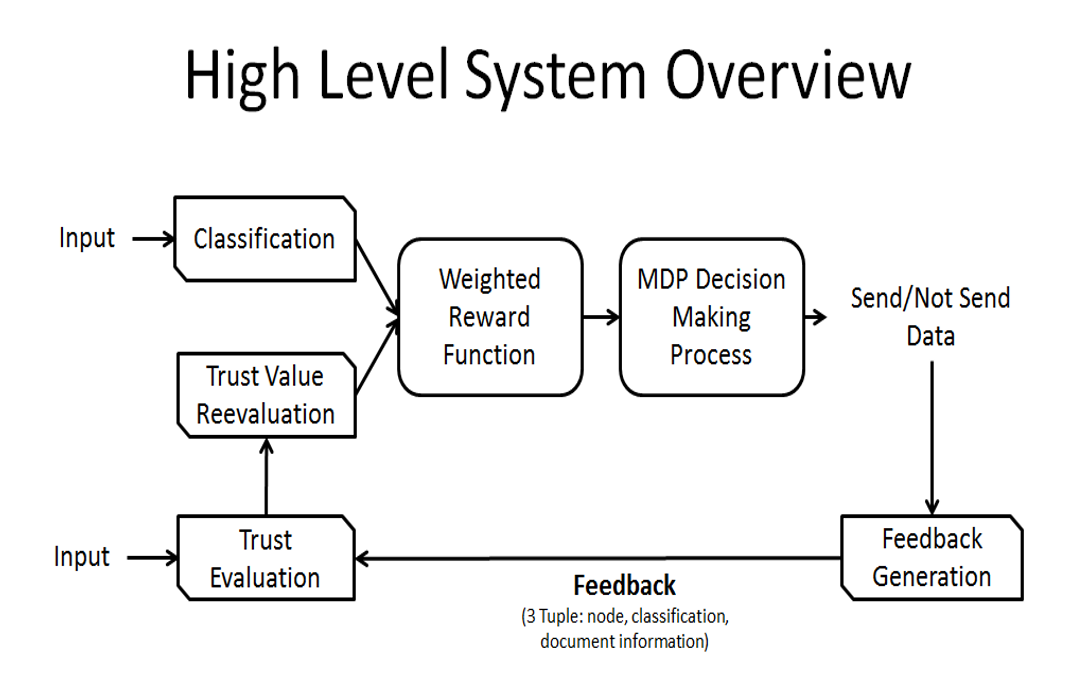
\includegraphics[width=0.90\textwidth]{Figures/HighLevelOverview.PNG}
        \caption{System Overview}
        \label{fig:SystemOverview}
    \end{center}
\end{figure}

\section{Background and Motivation}
A 2008 study commissioned by Cisco Systems of more than 2000 IT professionals in
10 countries revealed some startling statistics \autocite{Cisco2008}. Of these professionals,
39\% were more concerned about threats from their own employees, than from
malicious attackers outside of the company. The reason for this concern?
Almost half of the professionals questioned reported that in addition to
employees dealing with more information than ever before, and at a quicker
pace, they are also not receiving the proper education in data security
awareness. What this all adds up to is a shocking statistic: 11\% of the
professionals reported that either they or an employee they knew of, accessed
unauthorized information and sold it for profit. That is 1 out of every 10
employees. In a world where a source code file, design document, or other
digital file worth millions can be leaked via email, USB drive, internet,
etc., this creates a huge problem.  According to a May 2009 US federal
government report, between 2008 and 2009 American business losses due to
cyber-attacks have grown to more than \$1 trillion worth of intellectual
property \autocite{Cisco2008}. The impact of unauthorized data transmission can also go beyond
monetary damages. For example, the HBGary scandal resulted in the
imprisonment of several formerly successfully security professionals
\autocite{JiminLi2010}.
Thus a comprehensive data transfer mechanism is required to mitigate the
impact of unauthorized data transmission in cloud-based systems.

The problem of data leakage has yet to find a catch-all solution. Every day
millions of bits of data are transferred between users and computers in
organizations both large and small \autocite{Bright2012}. From losses that
include large sums of money, intellectual property, and even jail
sentences, the consequences of unauthorized data transmission can be massive.
Who is monitoring these data transmissions to protect against these? Obviously,
Software such as firewalls, policy checkers, virus scanners and others attempt to help
prevent this unauthorized transmission, but the software is often niche, focused
on one specific task, and proprietary. What if there was a system that could be
integrated into an organization, trained specifically to deal with a company�s
data, and provide security over the entire network. This is where our framework:
``CloudAssure'' comes into the picture. 

\section{Goals and Scope of Study of CloudAssure}
The objective of this project is to develop a data transfer decision framework
that makes informed decisions on data transmission among nodes (users) in
a cloud-based system. Here we refer to the concept of a cloud system as an interconnected network.
For the CloudAssure framework, a three part process is used; classification of data sensitivity,
dynamic trust evaluation, and real-time decision modeling. The goals that met with
our project in order to work achieving the aforementioned objective were
as follows: 
\begin{enumerate}
    \item Development of an effective framework to address unauthorized
        data transmission monitored by security agents which enact and enforce data
        transmission decisions in order to prevent and/or mitigate unauthorized data
        transmission in cloud-based systems.
    \item Development of a planning model using a \gls{mdp} to make a decision on whether to transmit data or not.
    \item Development of a standardized classification algorithm to aid security
        agents running the \gls{mdp} in making data transmission decisions among nodes
        by assessing the sensitivity of the data to be transferred in cloud
        environments.  
    \item Development of a Trust Evaluation Equation to aid the
    planning
        methodology in making a transmission decision.  The scope of this
        project is the generation of a theoretical model to make decisions based
        on dynamic trust values obtained from continuous node evaluation and the
        sensitivity of data obtained from the data classification stage. If
        possible, we would like to develop a practical implementation of our
        proposed classification algorithm. We assume the following:
        \begin{enumerate}
            \item We assume that the system periphery is adequately protected (no outsider attacks)
            \item There is an organizational structure (hierarchy) within the workforce.
            \item One time critical data leak prevention is not within our threat model.
            \item We assume the user identity/system is not compromised by a malicious actor.
        \end{enumerate}
\end{enumerate}

\begin{table}[h!]
    \centering
    \begin{tabular}{c | c | c | c}
        \hline
        Milestone	   &     Date	   &  Description   & Person \\
        \hline \hline
                       &     2/6/2013  &    Project Proposal Approved   &   \\
        Task 1 Complete&     2/14/2013 &	System Goals Decided   &   \\
                       &     2/18/2013 &	High-Level System Structure Initial Design Complete   &   \\
        Task 2 Complete&     2/21/2013 &	High-Level System Structure decided   &   \\
        Task 4 Complete&     2/26/2013 &	Planning Stage finalized   &   \\
        Task 3 Complete&     2/28/2013 &	Classification Stage finalized   &   \\
        Task 2 Complete&     2/28/2013 &	Trust Evaluation Stage finalized   &   \\
                       &     3/5/2013  &	Interim Progress Report Submitted   &   \\
                       &     4/1/2013  &    System refinement and finalization phase   &   \\
                       &     4/4/2013  &	Final Group Report Submitted   &   \\
                       &     4/9/2013  &	Class Presentation Slides Submitted   &   \\
                       &     4/9/2013  &	In Class Presentation   &   \\
    \end{tabular}
    \caption{Group Member Responsibilities}
\end{table}
